\newpage
\chapter{Tinjauan Pustaka} \label{Bab II}

\section{Tinjauan Pustaka} \label{II.Tinjauan}
Pada penelitian ini, peneliti melakukan eksplorasi dan mendapatkan tinjauan pustaka berdasarkan penelitian sebelumnya yang berkaitan dengan pembangunan model pendeteksi penipuan kartu kredit. Peneliti menjadikan penelitian terdahulu sebagai referensi dan landasan perbandingan serta kajian terhadap penelitian yang akan dilakukan. Berikut penelitian-penelitian terdahulu yang berhubungan dengan penelitian ini:
\begin{enumerate}[noitemsep]
	\item Tahun 2021, Asha RB, Suresh Kumar KR,       melakukan penelitian terkait dengan \textit{Credit card fraud detection using artificial neural network}. Tujuan Penelitian ini ialah untuk membandingkan hasil dari traditional machine learning seperti SVM dan ANN. Hasil dari penelitian ini ialah menunjukan bahwa ANN lebih baik dibandingkan traditional machine learning berdasarkan accuracy \cite{asha2021credit}.
    \item Tahun 2021, Tayebi, Mohammed dan El Kafhali, melakukan penelitian terkait dengan \textit{Hyperparameter optimization using genetic algorithms to detect frauds transactions}. Tujuan penelitian ini bertujuan untuk menangani penipuan transaksi kartu kredit dengan menggunakan \textit{machine learning} untuk mendeteksi penipuan dengan menerapkan \textit{genetic algorithm}(GA) untuk mengoptimalkan hyperparameter dan melakukan komparasi dengan menggunakan \textit{grid search method}. Evaluasi yang digunakan ialah \textit{accuracy}, precision, \textit{recall}, dan \textit{F1 score}\cite{tayebi2021hyperparameter}.
    \item Tahun 2022, Putu Tirta Sari Ningsih, Muhammad Gusvarizon, Rudi Hermawan, melakukan penelitian terkait dengan Analisis sistem pendeteksi penipuan transaksi kartu kredit dengan algoritma machine learning. Tujuan penelitian ini ialah melakukan komparasi berbagai algoritma \textit{machine learning} seperti \textit{decision tree}, \textit{random forest}, \textit{logistic regression}, dan \textit{support vector machine} dalam membuat sistem pendeteksi penipuan transaksi kartu kredit. Evaluasi yang digunakan ialah \textit{accuracy}, \textit{precision}, \textit{recall}, \textit{F-1 score}, \textit{receiver operating characteristics}(ROC), \textit{area Under the Curve}(AUC), dan \textit{matthew coefficient score}(MCC). Hasil penelitian ini membuktikan ensemble learning algoritm seperti random forest merupakan algoritma terbaik dalam membuat sistem pendeteksi penipuan transaksi kartu kredit karena memiliki nilai performa keseluruhan paling baik dengan MCC 87\%\cite{ningsih2022analisis}.
    \item Tahun 2022, Kumar Sheo, Gunjan Vinit Kumar, Ansari Mohd Dilshad, Pathak, Rashmi, melakukan penelitian terkait dengan \textit{Credit card fraud detection using support vector machine}. Tujuan riset ini ialah menemukan sistem paling efektif dalam mengidentifikasi penipuan kartu kredit dengan menggunakan \textit{support vector machine} dalam  menglasifikasi penipuan dan normal transaksi kartu kredit dalam melakukan deteksi.\cite{kumar2022credit}.
    \item Tahun 2020, Ruttala Sailusha, V. Gnaneswar, R. Ramesh, dan G. Ramakot eswara Raom, melakukan penelitian terkait dengan \textit{Credit card fraud detection using machine learning}. Penelitian ini membandingkan dua algoritma \textit{ensemble learning} yaitu \textit{random forest} dan \textit{adaboost}. Evaluasi yang digunakan ialah \textit{accuracy}, \textit{precision}, \textit{recall}, \textit{F-1 score}. Hasil dari penelitian ini memberikan kesimpulan kalau walaupun banyaknya teknik deteksi penipuan dia tidak bisa bilang kalau algoritma bisa mendeteksi penipuan secara menyeluruh dan hasil komparasinya menunjukan kalau secara akurasi \textit{random forest} dan \textit{adaboost} menunjukan kesamaan namun secara \textit{precision}, \textit{recall}, \textit{F-1 score} \textit{random forest} lebih unggul. \cite{9121114}.
    \item Tahun 2024, Abdul Rehman Khalid, Nsikak Owoh, Omair Uthmani, Moses Ashawa, Jude Osamor, dan John Adejoh, melakukan penelitian terkait \textit{Enhancing credit card fraud detection: an ensemble machine learning approach}. Tujuan penelitian ini melakukan komparasi analisis terkait \textit{ensemble machine learning} seperti \textit{support vector machine} \textit{random forest} dan \textit{boosting classifiers}. Hasil dari penelitian ini mengaris bawahi bahwa ensemble methods merupakan tool yang terbaik untuk menangani kasus penipuan transaksi. \cite{khalid2024enhancing}
    \item Tahun 2023, Purwar, Archana and Manju, Ms, melakukan penelitian terkait \textit{Credit card fraud detection using XGBoost for imbalance dataset}. Tujuan dari penelitian ini ialah membuat model pendeteksi transaksi penipuan kartu kredit dengan menggunakan \textit{learning algorithm} xgboost. Hasil penelitian ini menunjukan bahwa xgboost menghasilkan performa model yang baik. \cite{purwar2023credit}
\end{enumerate}

\begin{longtable}{| b{0.05\textwidth}|p{0.2\textwidth}|p{0.2\textwidth}|p{0.15\textwidth}|p{0.25\textwidth}|} % Longtable berguna agar tabel dapat terpotong di halaman baru
	\caption{Literasi Penelitian Terdahulu}
	\label{table:2.literasi}\\
	\hline
	\textbf{No.} & \textbf{Judul} & \textbf{Masalah} & \textbf{Metode} & \textbf{Hasil} \\
	\hline
	\endhead % Agar semua baris diatas ini diulang jika melewati halaman baru (repeat header row)
	1. & \textit{Credit card fraud detection using artificial neural network}  & Penipuan dalam transaksi kartu kredit merupakan hal yang umum saat ini karena sebagian besar dari kita lebih sering menggunakan metode pembayaran kartu kredit. Hal ini disebabkan kemajuan teknologi dan peningkatan transaksi online mengakibatkan penipuan yang menyebabkan kerugian finansial yang sangat besar. & support vector machine (SVM),  k-nearest neighbor (KNN), Artificial neural network (ANN) & SVM accuracy= 0.9349 precision= 0.9743 recall= 0.8976, KNN accuracy= 0.9982 precision= 0.7142 recall= 0.0393, dan ANN accuracy= 0.9992 precision= 0.8115 recall= 0.7619\\ 
	\hline
	2. & \textit{Hyperparameter optimization using genetic algorithms to detect frauds transactions} & sekarang servis online berkembang menjadi sangat besar dan maka dengan itu juga penipuan dalam servis online juga menjadi lebih besar, termasuk penipuan traksasi kartu kredit. & SMOTE, grid search (GS) methods, random forest (RF),
    AdaBoost (AB), logistic regression (LR), decision tree (DT), and support vector machine (SVM) classifier. & SVM: Precision=95\%, Recall=95\%, F1-score=95\%, Accuracy=94\%, Time=19.039
    LR: Precision=97\%, Recall=91\%, F1-score=94\%, Accuracy=94\%, Time=104.016
    AB: Precision=98\%, Recall=93\%, F1-score=95\%, Accuracy=95\%, Time=235.037
    RF: Precision=96\%, Recall=92\%, F1-score=94\%, Accuracy=94\%, Time=130.300
    DT: Precision=94\%, Recall=91\%, F1-score=93\%, Accuracy=92\%, Time=12.709\\ 
	\hline
	3. & Analisis sistem pendeteksi penipuan transaksi kartu kredit dengan algoritma machine learning & Banyaknya volume transaksi dan cepatnya proses transaksi yang berlangsung, membuat tidak mungkin untuk diawasi secara manual oleh manusia karena itu penpuan transaksi menjadi masalah dan harus diselesaikan dengan machine & analisis komparasi model + imbalance, model + SMOTE, model + param + imbalance, model + param + SMOTE, dengan model decision tree (DT), random forest (RF), logistic regression (LR), dan support vector machine (SVM) & algoritma random forest (RF) memiliki performa paling baik di antara semua model,
    disusul oleh model dengan algoritma decision tree (DT), hal ini pula yang membuktikan
    bahwa ensemble learning adalah teknik terbaik untuk fraud detection.\\ 
	\hline
    4. & \textit{Credit card fraud detection using support vector machine} & Penipuan kartu kredit tidak diragukan lagi merupakan ekspresi penipuan kriminal. Identifikasi penipuan tampaknya menjadi masalah rumit yang memerlukan banyak keterampilan hingga memasukkan algoritma terkait pembelajaran mesin ke dalamnya. & SVM &  Hasil simulasi menunjukan bahwa SVM lebih baik dibandingkan \textit{state of art approaches}. \\
    \hline
    5. & \textit{Credit card fraud detection using machine learning} & Deteksi penipuan kartu kredit saat ini paling banyak dilakukan
    karena permasalahannya yang sering terjadi di dunia saat ini. hal ini disebabkan
    peningkatan transaksi online dan platform e-commerce & Adaboost dan Random Forest & Random Forest precision= 0.97\% recall= 89\% f1-score= 0.93 AUC=94\%, Adaboost precision= 89\% recall= 81,5\% f1-score= 84,5\% AUC=96\%.\\
    \hline
    6. & \textit{Enhancing credit card fraud detection: an ensemble machine learning approach} & Di era kemajuan digital, meningkatnya penipuan kartu kredit mengharuskan adanya pengembangan sistem deteksi penipuan yang kuat dan efisien. & Membandingkan ensemble learning dan traditional machine learning Support Vector Machine
    (SVM), K-Nearest Neighbor (KNN), Random Forest (RF), Bagging, and Boosting classifiers.) & Metode ensamble mengungguli model individual, menunjukkan efektivitas penggabungan beberapa model. \\
    \hline
    7. & \textit{Credit card fraud detection using XGBoost for imbalanced data set} & peningkatan tingkat penipuan di seluruh dunia, berbagai algoritma pembelajaran mesin digunakan oleh analis dan peneliti untuk mendeteksi dan menganalisis penipuan dalam transaksi online. Namun, kumpulan data pelatihan mungkin memiliki beberapa instance dari satu atau lebih instance dari kelas lain dalam kasus klasifikasi biner kelas tertentu yang membuat hasilnya menjadi bias. & XGBOOST & F1 score, recall and accuracy as 82.78\%, 78.9\% and 99.3\% \\
    \hline
\end{longtable}

\section{Dasar Teori} \label{II.Teori}
\subsection{Machine Learning} \label{II.Dasar Teori}
\textit{Machine learning} merupakan sebuah algoritma yang dapat membuat komputer belajar tanpa diprogram secara langsung\cite{alpaydin2021machine}. Kemampuan untuk belajar dan menentukan pilihan berdasarkan hasil pembelajaran, membuat \textit{Machine Learning} sering disebut sebagai AI atau \textit{Artificial Intelligence}. Namun, kenyataannya itu merupakan sub divisi dari AI dan pada tahun 1970an baru menjadi bagian dari evolusi AI dikarenakan sebelum tahun tersebut peneliti lebih berfokus kepada pendekatan \textit{logical} dan \textit{knowledge-based} dibandingkan algoritma dan juga lambatnya komputer dimasa lalu berdampak dalam performa \textit{machine learning} yang membuat banyak peneliti tidak berfokus meneliti hal tersebut\cite{fradkov2020early}. \textit{Machine Learning} menjadi salah satu algoritma yang sangat penting dalam membantu perkembangan industri dikarenakan kemampuan automasinya yang bisa terus berkembang\cite{jordan2015machine}. \textit{Machine learning} terus membesar dan bisa digunakan di dalam sebuah \textit{e-commerce}, \textit{social media}, medis, bank dan lain-lain\cite{jordan2015machine}.\\
Algoritma \textit{machine learning} dibuat dengan model matematika yang dijalankan di sebuah komputer yang diberikan inputan data atau biasa disebut \textit{training data} untuk membuat sebuah keputusan tanpa secara khusus diprogram langsung oleh \textit{programmer} untuk membuat keputusan\cite{alpaydin2021machine}.

\subsection{Supervised Learning} \label{II.Supervised Learning}
\textit{Supervised Learning} ialah salah satu tipe \textit{machine learning} di mana algoritma dilatih menggunakan data yang sudah memiliki label atau kelas yang diketahui. \textit{Supervised learning} berlandaskan sebuah \textit{input} data dan memberikan \textit{output} berupa label label seperti pada gambar \ref{fig:2.carasupervised}\cite{cunningham2008supervised}.
\begin{figure}[H] % Kalau menggunakan H, posisi gambar akan tepat dibawah teks
    \centering
    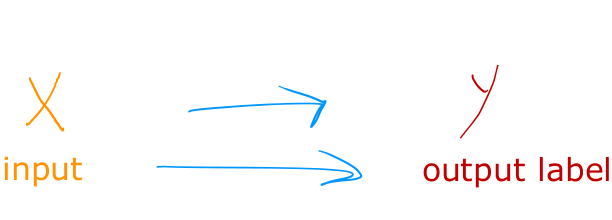
\includegraphics[width=0.8\textwidth]{figure/image.png}
    \caption{Cara Kerja Supervised Learning}
    \label{fig:2.carasupervised}
\end{figure}
\textit{Supervised learning} dibagi menjadi dua ranah dalam \textit{machine learning} yaitu klasifikasi dan regresi\cite{cunningham2008supervised}. Algoritma Klasifikasi digunakan untuk membuat prediksi berdasarkan kategori yang ditentukan yang artinya memiliki jumlah kemungkinan \textit{output} yang kecil, contohnya algoritma untuk memprediksi penipuan kartu kredit karena mengklasifikasi 2 kemungkinan yaitu transaksi penipuan dan transaksi normal \cite{cunningham2008supervised}. Algoritma Regresi merupakan sebuah algoritma yang mendeteksi nilai yang berkelanjutan, contohnya seperti sistem prediksi kenaikan harga saham karena memungkinkan untuk memiliki banyak kemungkinan \textit{output} untuk mengetahui hasil prediksinya\cite{cunningham2008supervised}. 


\subsection{\textit{Gradient Descent}} \label{II.Gradient Descent}
\textit{Gradient descent} merupakan sebuah \textit{optimization algorithm} yang umum digunakan untuk melatih model \textit{machine learning} dan \textit{neural networks}\cite{hochreiter2001learning}. \textit{Gradient descent} melatih \textit{machine learning} models dengan minimalisasi errors antara hasil prediksi dan nilai asli dengan mengganti parameter w dan b\cite{hochreiter2001learning}.\\
\textit{Cost function} merupakan cara untuk mengetahui performa dari sebuah model, dengan cara mengurang \textit{output} hasil prediksi dengan hasil sebenarnya untuk mendapatkan nilai akurasi, semakin kecil keluaran nilai dari \textit{cost function} maka akurasi semakin baik\cite{alpaydin2021machine}. Contohnya dalam model \textit{linear regression} yang mempunyai rumus untuk modelnya dalam bentuk seperti ini  $y = wx + b$ yang mana $y = f_{w,b}(x)$ maka formula dari cost function menjadi seperti ini.\\
\begin{equation}
    J(w,b) = \frac{1}{2m} \sum\limits_{i = 0}^{m-1} (f_{w,b}(x^{(i)}) - y^{(i)})^2
\end{equation}
\label{eq:2.CostFunction}
\myequations{Rumus Cost Function}
\\
dengan diketahui bahwa:
\begin{center}
$J(w,b)$ = \textit{cost function} dengan parameter w dan b\\
$w$ = slope / turunan\\
$b$ = \textit{y-axis intercept}\\
$m$ = jumlah data training\\
$y$ = nilai sebenarnya\\
$f_w,_b$ = nilai prediksi\\
$i$ = nilai iterasi\\
\end{center}

\subsubsection{Perhitungan \textit{Cost Function}} \label{II.costfunction}
Perhitungan \textit{cost function} untuk membuat sebuah model prediksi \textit{linear regression} dengan dataset sederhana dengan jumlah 2 data dengan fitur x dan y. Data pertama x = 1 dan y = 300 dan data kedua x = 2 dan y = 500.\\ 
Perhitungan cost function digunakan untuk mengetahui gambaran performa dari sebuah model dengan inputan w dan b tertentu. Contoh inputkan w = 150, b = 100 dan nilai x yang di inputkan ke dalam sebuah model \textit{linear regression} $y = wx + b$ dan setelah itu hitung cost functionnya.\\
Hasil dari \textit{cost function} w = 150 dan b = 100 adalah 3.125 yang tergambarkan dengan grafik \textit{scatter plot} untuk y dan x seperti pada gambar \ref{fig:2.scatterplotlinear}.
\begin{figure}[H] % Kalau menggunakan H, posisi gambar akan tepat dibawah teks
    \centering
    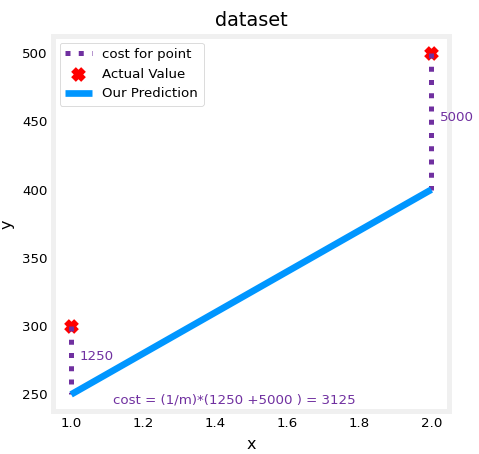
\includegraphics[width=0.5\textwidth]{figure/scatter plot linear regression.png}
    \caption{Scatter Plot Linear Regression}
    \label{fig:2.scatterplotlinear}
\end{figure}
Grafik \textit{scatter plot} tersebut menunjukan bahwa hasil \textit{cost function} w = 150 dan b = 100 belum menghasilkan \textit{output} yang baik dikarenakan \textit{straight line} belum \textit{fit} kedalam data dan bisa dilihat pada gambar \ref{fig:2.scatterplotcost} dan nilai w yang belum mencapai nilai \textit{local minimum}.
\begin{figure}[H] % Kalau menggunakan H, posisi gambar akan tepat dibawah teks
    \centering
    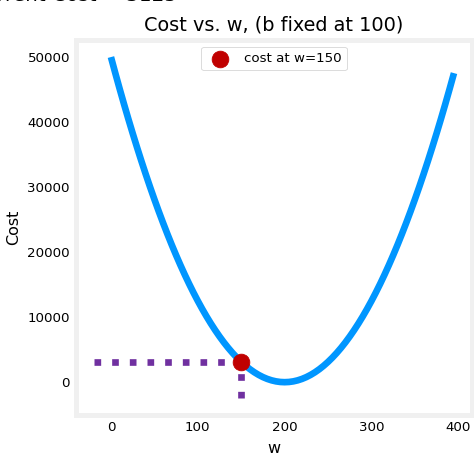
\includegraphics[width=0.5\textwidth]{figure/Scatter plot cost function.png}
    \caption{Scatter Plot Cost Function}
    \label{fig:2.scatterplotcost}
\end{figure}

\subsubsection{Cara Kerja \textit{Gradient Descent}} \label{II.carakerjagradientdescent}
\textit{Gradient descent} merupakan algoritma yang digunakan untuk terus mengubah w dan b untuk mengurangi $j(w,b)$ sampai akhirnya mencapai \textit{local minimum}\cite{hochreiter2001learning}. Analoginya ialah seperti pendaki yang ingin turun bukit namun banyak kabut disekitarnya sehingga dia tidak bisa melihat contohnya seperti pada gambar \ref{fig:2.gradientdescent}.
\begin{figure}[H] % Kalau menggunakan H, posisi gambar akan tepat dibawah teks
    \centering
    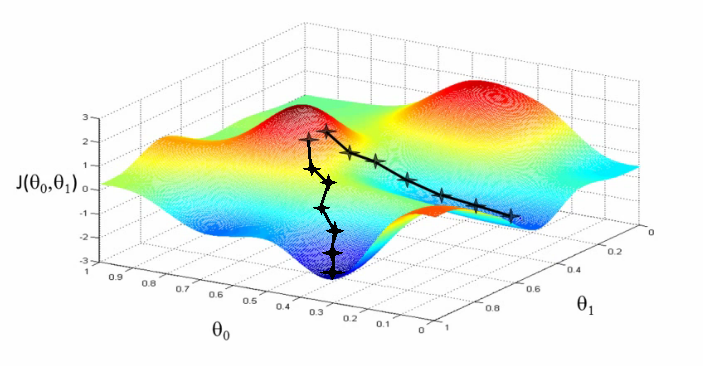
\includegraphics[width=0.5\textwidth]{figure/gradient descent.png}
    \caption{Gradient Descent}
    \label{fig:2.gradientdescent}
\end{figure}
Seperti yang terlihat pada gambar \ref{fig:2.gradientdescent}. pendaki akan mencoba untuk mencari cara untuk turun ke dasar dengan cara mengecek sekelilingnya dan setelah itu mencoba untuk melangkah satu kali dan setelah itu mengecek apakah langkah tersebut membuatnya turun atau tidak, jika turun maka pendaki akan mencoba untuk melangkah ke arah yang sama dan jika tidak maka pendaki mencoba langkah yang berbeda dan ada hal perlu diperhatikan pada gambar \ref{fig:2.gradientdescent} yang menunjukan bahwa local minimum bisa terdapat lebih dari 1\cite{ruder2016overview}.\\
Gradient descent memiliki formula seperti cost function untuk menjalankan sebuah algoritma nya untuk mengganti nilai w dan b agar bisa mencapai \textit{local minimum}.\\
Formula gradient descent\cite{ruder2016overview}: \\
\begin{equation}
\text{repeat until convergence: } 
\left\lbrace
\begin{aligned}
  w &= w - \alpha \frac{\partial J(w,b)}{\partial w} \\
  b &= b - \alpha \frac{\partial J(w,b)}{\partial b}
\end{aligned}
\right.
\end{equation}
\label{eq:2.gradient}
\myequations{Rumus Gradient Descent}
\\
yang diketahui bahwa:
\begin{center}
    $\alpha$ = \textit{Learning rate}\\
    $\partial$ = \textit{Partial derivative}
\end{center}
Yang mana parameter w dan b akan \textit{update simultaneously}.\\
Hasil dari \textit{partial derivative} dari $\frac{\partial J(w,b)}{\partial w}$ dan juga $\frac{\partial J(w,b)}{\partial b}$ seperti berikut. \\
\begin{equation}
    \begin{aligned}
    \frac{\partial J(w,b)}{\partial w} &= \frac{1}{m} \sum_{i=0}^{m-1} \left( f_{w,b}\left(x^{(i)}\right) - y^{(i)} \right) x^{(i)} \\
    \frac{\partial J(w,b)}{\partial b} &= \frac{1}{m} \sum_{i=0}^{m-1} \left( f_{w,b}\left(x^{(i)}\right) - y^{(i)} \right)
    \end{aligned}
\end{equation}
\label{eq:2.partialgradient}
\myequations{Hasil Partial Derivative Gradient}

\subsubsection{Learning Rate} \label{II.learningrate}
Learning Rate($\alpha$) merupakan salah satu parameter terpenting dalam \textit{machine learning} terkhusus dalam konteks \textit{gradient descent}\cite{igiri2015effect}. \textit{ Learning rate} menentukan ukuran langkah yang dapat diambil pada setiap iterasinya\cite{zeiler2012adadelta}. Menentukan \textit{learning rate} merupakan hal yang krusial dikarenakan jika \textit{learning rate} terlalu kecil maka gradient descent akan berjalan sangat lambat seperti pada gambar \ref{fig:2.learningratekecil} dan apabila nilai learning rate terlalu besar maka bisa terjadi \textit{overshoot} atau tidak pernah mencapai \textit{local minimum} seperti pada gambar \ref{fig:2.learningratebesar}\cite{igiri2015effect}.
\begin{figure}[H] % Kalau menggunakan H, posisi gambar akan tepat dibawah teks
    \centering
    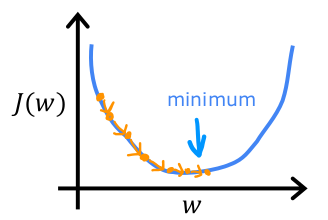
\includegraphics[width=0.5\textwidth]{figure/Learning rate kecil.png}
    \caption{Learning Rate Terlalu Kecil}
    \label{fig:2.learningratekecil}
\end{figure}
\begin{figure}[H] % Kalau menggunakan H, posisi gambar akan tepat dibawah teks
    \centering
    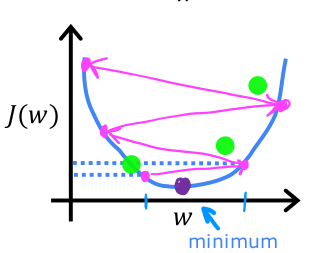
\includegraphics[width=0.5\textwidth]{figure/Learning rate besar.png}
    \caption{Learning Rate Terlalu Besar}
    \label{fig:2.learningratebesar}
\end{figure}
Ada berbagai cara untuk menentukan nilai learning rate terbaik salah satu cara paling umum dilakukan ialah dengan menggunakan \textit{grid search}, dengan \textit{grid search} kita bisa melakukan berbagai iterasi dengan nilai learning rate berbeda-beda dan lakukan analsis komparasi untuk menentukan nilai \textit{learning rate} terbaik\cite{smith2018disciplined}. Salah satu cara untuk memilih range nilai learning rate yang akan dimasukan ke grid search ialah dengan skala logaritmic contohnya dari $10^{-6}$ sampai $10^{-1}$\cite{smith2018disciplined}.


\subsection{Kartu Kredit} \label{II.KartuKredit}
Kartu kredit merupakan alat pembayaran nontunai yang memberikan fasilitas kredit kepada pemegang nya\cite{wooster1966credit}. Pemegang kartu kredit wajib membayar tagihan  akibat penggunaan kartu tersebut pada waktu yang  ditentukan dalam kontrak\cite{wooster1966credit}. Kewajiban pembayaran ini berlaku untuk seluruh transaksi yang dilakukan, termasuk pembelian barang dan jasa serta penarikan uang tunai\cite{flitcroft2009credit}. \\
Ada dua jenis transaksi  kartu kredit: transaksi \textit{card-present}(CP) dan transaksi \textit{card-not-present}(CNP)\cite{kumar2016method}. Transaksi \textit{card-present} terjadi ketika kartu kredit secara fisik digunakan di lokasi transaksi, misalnya saat berbelanja di toko dan menggesek kartu di mesin EDC. Sebaliknya, transaksi \textit{card-not-present} tidak memerlukan kehadiran fisik kartu, seperti saat berbelanja online atau melakukan pembayaran melalui telepon dan dalam transaksi CNP, data kartu kredit dimasukkan secara manual atau otomatis ke dalam sistem pembayaran\cite{kumar2016method}. Berikut merupakan contoh bagian-bagian yang ada pada sebuah kartu kredit.
\begin{enumerate}[noitemsep]
    \item \textit{Chip}  kartu kredit terletak di bagian depan kartu. \textit{Chip} ini ditambahkan pada berbagai aplikasi yang dapat mengenkripsi data agar dapat disimpan dengan lebih aman.
    \item  Nomor kartu adalah 16 digit nomor kartu kredit. Nomor ini tidak akan pernah sama dengan nomor kartu kredit lainnya.
    \item \textit{Cardholder Name} adalah nama  pemilik atau pemegang kartu kredit.
    \item Nama atau logo penerbit adalah nama atau logo perusahaan penerbit kartu.
    \item Masa berlaku adalah tanggal dalam format dua digit setelah bulan dan tahun  masa berlaku kartu kredit.
    \item Logo jaringan kartu (GPN pada diagram) adalah logo jaringan kartu kredit.
    \item Terdapat strip magnet di bagian belakang yang dapat dibaca dengan menggesek kartu saat bertransaksi.
    \item Tanda tangan pemegang kartu dimasukkan pada kolom tanda tangan.
    \item  Nomor verifikasi atau CVV/CVC adalah 3 digit angka di sebelah kolom tanda tangan.
    \item Alamat bank penerbit adalah alamat perusahaan/bank yang menerbitkan kartu.
    \item  Nama atau logo penerbit kartu.
\end{enumerate}
\begin{figure}[H] % Kalau menggunakan H, posisi gambar akan tepat dibawah teks
    \centering
    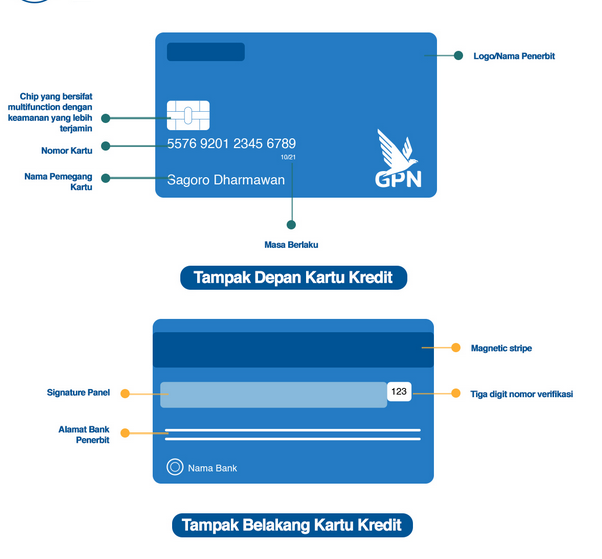
\includegraphics[width=0.5\textwidth]{figure/kartu.png}
    \caption{Kartu Kredit}
    \label{fig:2.kartukredit}
\end{figure}

\subsection{\textit{Imbalanced data}} \label{II.Imbalanced Data}
\textit{Imbalanced data} merupakan sebuah kondisi di sebuah data di mana jumlah data antara kelas satu dan lainnya tidak seimbang yang artinya salah satu kelas memiliki jumlah yang lebih besar dibandingkan lainnya\cite{haixiang2017learning}. \textit{Imbalanced dataset} kemunculannya merupakan hal alami yang akan selalu muncul pada kejadian yang langka, namun kejadian langka tersebut bisa menyebabkan hal buruk apabila terjadi, salah satu contohnya ialah  pada data transaksi penipuan, data penyakit kanker\cite{krawczyk2016learning}. Kejadian langka tersebut dapat mengakibatkan kerugian besar apabila terjadi dan dibutuhkan sistem yang bisa memprediksi kejadian langka tersebut\cite{krawczyk2016learning}.\\
\textit{Imbalanced dataset} merupakan masalah yang besar di sebuah\textit{ machine learning} dikarenakan dapat mengakitbatkan bias yang cenderung lebih ke kelas mayoritas. hal ini membuat model menjadi sulit untuk mendeteksi kelas dengan jumlah lebih sedikit atau minoritas\cite{haixiang2017learning}. Berikut ini merupakan visualisasi \textit{imbalanced data} yang dapat dilihat pada gambar \ref{fig:2.visualisasiimbalanced}.
\begin{figure}[H] % Kalau menggunakan H, posisi gambar akan tepat dibawah teks
    \centering
    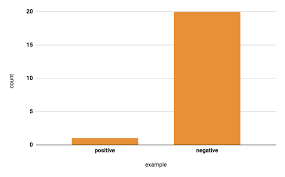
\includegraphics[width=0.5\textwidth]{figure/gambar imbalance data.png}
    \caption{Visualisasi Imbalanced Data}
    \label{fig:2.visualisasiimbalanced}
\end{figure}

\subsection{\textit{Hyperparameter}} \label{II.hyperparameter}
\textit{Hyperparameter} adalah parameter yang ditentukan sebelum proses pelatihan model pembelajaran mesin dimulai\cite{yang2020hyperparameter}. Berbeda dengan parameter model, yang dipelajari secara otomatis selama pelatihan, \textit{hyperparameter} memengaruhi cara model mempelajari dan mengambil keputusan\cite{bischl2023hyperparameter}. Contoh \textit{hyperparameter} ialah:
\begin{enumerate}[noitemsep]
    \item \textit{Learning rate}.
    \item jumlah iterasi.
    \item jumlah \textit{tree} dalam \textit{ensemble methods}.
    \item kedalaman \textit{tree} dalam \textit{decision tree}.
    \item jumlah \textit{neuron} dalam \textit{neural network}.
\end{enumerate}
\textit{Hyperparameter} berguna dalam membangun strutur dan kompleksitas dari model \textit{machine learning}. Pemilihan \textit{hyperparameter} yang tepat dapat sangat mempengaruhi kinerja model\cite{bischl2023hyperparameter}. Cara menentukan \textit{hyperparameter} bisa dilakukan dengan berbagai cara seperti berikut ini.\cite{yang2020hyperparameter}:
\begin{enumerate}[noitemsep]
    \item \textit{Grid Search}
    \item \textit{Random Search}
    \item \textit{Bayesian Optimization}
    \item \textit{Manual Tuning}
    \item \textit{Automated Hyperparameter Tuning(seperti Optuna)}
\end{enumerate}

\subsection{Feature Engineering} \label{II.featureengineering}
\textit{Feature engineering} adalah proses penting dalam \textit{machine learning} yang melibatkan pemilihan, modifikasi, atau penciptaan fitur (variabel input) yang membantu sebuah model untuk belajar\cite{alpaydin2021machine}. Tujuan dari \textit{feature engineering} adalah untuk meningkatkan performa model dengan menyediakan representasi data yang lebih baik\cite{alpaydin2021machine}.   

\subsubsection{Feature Creation} \label{II.featurecreation}
Feature creation merupakan salah satu tipe \textit{feature engineering} yang mana fitur-fitur atau variabel-variabel baru diciptakan berdasarkan data yang sudah ada\cite{alpaydin2021machine}. Tujuannya adalah untuk menyediakan informasi tambahan yang mungkin tidak langsung tersedia dalam data mentah, tetapi bisa membantu model pembelajaran mesin dalam membuat prediksi yang lebih akurat\cite{dong2018feature}. Salah satu contoh kegunaan dari feature creation adalah dalam mengenali sebuah ciri-ciri tertentu yang digunakan untuk membuat sistem prediksi, seperti ingin prediksi harga sebuah rumah berdasarkan data panjang dan lebar, dengan data tersebut kita bisa membuat fitur baru seperti luas dengan mengalikan panjang dan lebar. Contoh visualisasi dalam kasus ini ialah saat kita memiliki data yang memiliki fitur panjang dan lebar dan mencoba untuk dimasukan kedalam sebuah model machine learning dan ternyata hasil dari model machine learning belum bisa dikatakan baik seperti pada gambar \ref{fig:2.visualisasisebelumfeaturecreation}. Dalam hal ini kita mungkin harus mencoba membuat feature creation baru agar dapat menghasilkan hasil model machine learning yang lebih baik dengan membuat feature creation luas dan ternyata hasil dari machine learning menjadi lebih baik seperti pada gambar \ref{fig:2.visualisasisesudahfeaturecreation}.

\begin{figure}[H] % Kalau menggunakan H, posisi gambar akan tepat dibawah teks
    \centering
    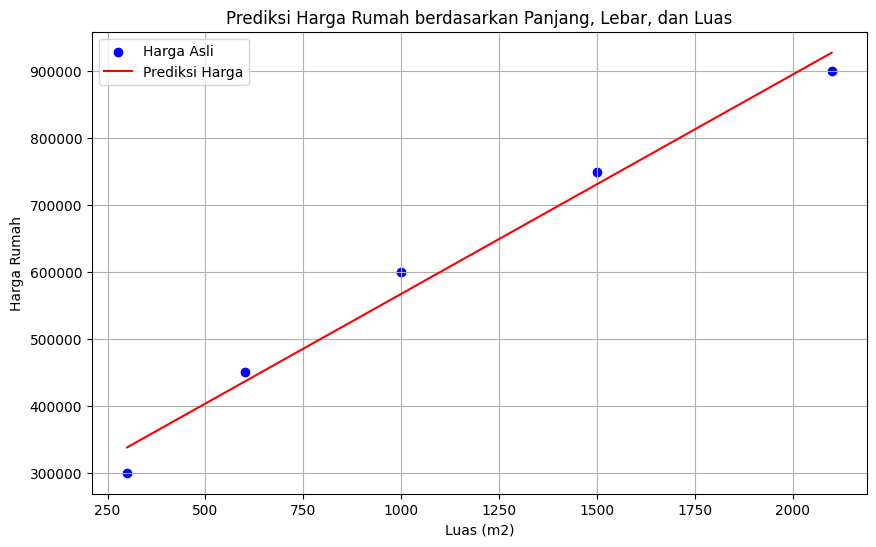
\includegraphics[width=0.5\textwidth]{figure/output feature creation only one feature.png}
    \caption{Visualisasi Sebelum Feature Creation}
    \label{fig:2.visualisasisebelumfeaturecreation}
\end{figure}

\begin{figure}[H] % Kalau menggunakan H, posisi gambar akan tepat dibawah teks
    \centering
    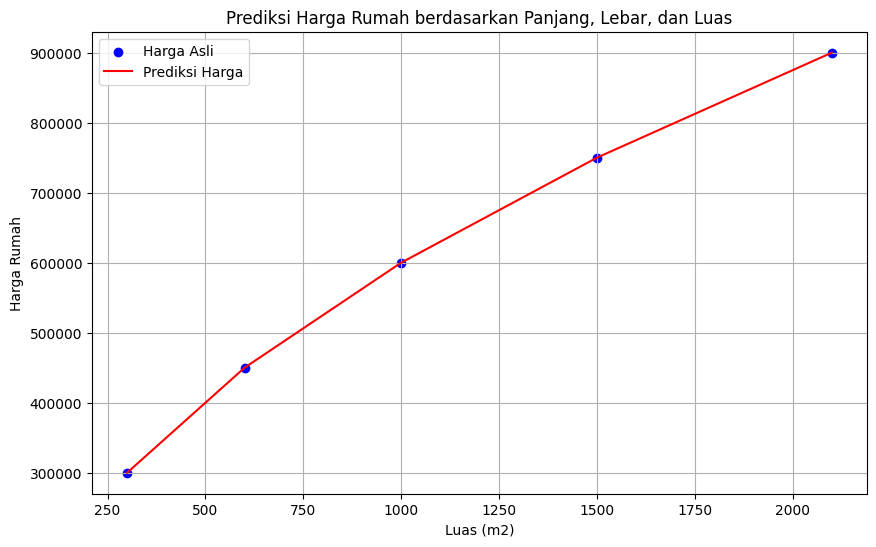
\includegraphics[width=0.5\textwidth]{figure/output feature creation multiple feature.png}
    \caption{Visualisasi Sesudah Feature Creation}
    \label{fig:2.visualisasisesudahfeaturecreation}
\end{figure}
Hasil dari visualiasi diatas menunjukan kalau feature creation dapat meningkatkan kemampuan model dalam belajar namun setelah mengetahui hal tersebut diperlukan pertimbangan agar tidak terjadi overfitting saat melakukan feature creation.

\subsubsection{Feature Scaling} \label{II.featurescaling}
\textit{Feature scaling} adalah sebuah proses untuk mengubah rentang nilai fitur dalam sebuah \textit{dataset} menjadi seimbang atau dengan skala yang sama\cite{alpaydin2021machine}. Hasil proses \textit{feature scaling} sangat penting dalam \textit{machine learning} dikarenakan untuk menghindari sensitivitas dalam algoritma yang membuat ada sebuah fitur mendominasi fitur lainnnya\cite{dong2018feature}. Feature Scaling juga mempengaruhi bagaimana algoritma \textit{gradient descent} bekerja, dengan memiliki skala yang tidak seimbang maka akan membuat \textit{gradient descent} menjadi lebih lama dalam menemukan \textit{local minimum} atau bahkan tidak menemukannya sama sekali\cite{ruder2016overview}. Cara melakukan \textit{feature scaling} dalam python ialah dengan menggunakan \textit{library} \textit{scikit-learn} terkait \textit{preprocessing}. Hasil dari \textit{feature scaling} ialah membuat rentang nilai antara fitur satu dan lainnya menjadi lebih setara seperti pada gambar \ref{fig:2.visualisasisebelumfeaturescaling} menunjukan bahwa fitur 2 dan fitur 3 mempunyai rentang nilai yang sangat berbeda, dan setelah melakukan \textit{feature scaling} seperti pada gambar \ref{fig:2.visualisasisesudahfeaturescaling} menunjukan bahwa rentang nilainya menjadi lebih seimbang.
\begin{figure}[H] % Kalau menggunakan H, posisi gambar akan tepat dibawah teks
    \centering
    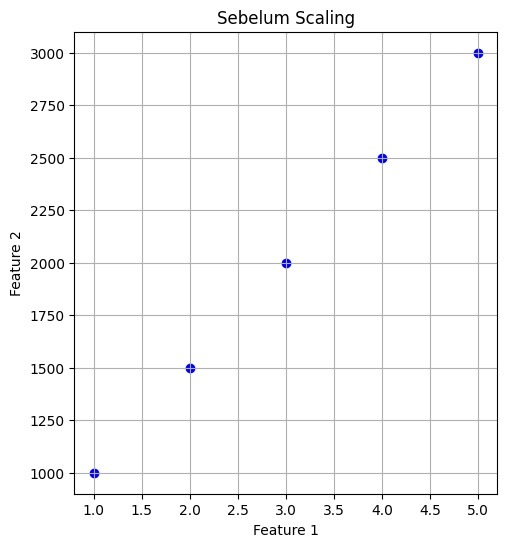
\includegraphics[width=0.5\textwidth]{figure/before feature scaling.png}
    \caption{Visualisasi Sebelum Feature Scaling}
    \label{fig:2.visualisasisebelumfeaturescaling}
\end{figure}
\begin{figure}[H] % Kalau menggunakan H, posisi gambar akan tepat dibawah teks
    \centering
    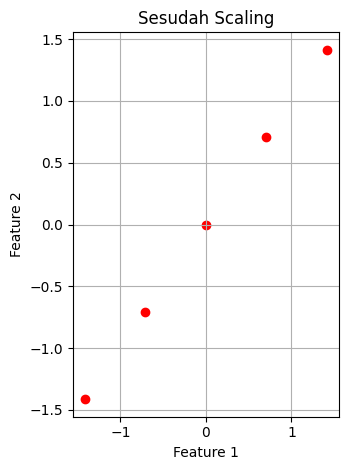
\includegraphics[width=0.5\textwidth]{figure/after feature scaling.png}
    \caption{Visualisasi Sesudah Feature Scaling}
    \label{fig:2.visualisasisesudahfeaturescaling}
\end{figure}
Dari contoh diatas dapat dilihat bahwa rentang nilai dari fitur satu dan fitur dua menjadi lebih seimbang yang artinya membuat machine learning untuk belajar dengan hasil yang lebih baik

\subsection{\textit{Oversampling}} \label{II.oversampling}
\textit{Oversampling} adalah teknik yang digunakan dalam \textit{machine learning} dan analisis data untuk menangani masalah \textit{unbalanced} data dalam dataset\cite{liu2004effect}. \textit{Unbalanced data} muncul ketika terdapat satu kelas atau fitur yang memiliki jumlah data sampel yang jauh lebih banyak dibandingkan kelas atau fitur lainnya\cite{dal2015calibrating}. Contohnya, dalam \textit{dataset} untuk mendeteksi penipuan kartu kredit, total jumlah transaksi yang normal mungkin jauh lebih banyak daripada jumlah transaksi penipuan.\\
Tujuan dari \textit{oversampling} ialah untuk membuat data menjadi \textit{balance} atau seimbang agar saat diinputkan ke \textit{machine learning}, model tidak menjadi bias terhadap kelas mayoritas. Salah satu contoh dari metode \textit{oversampling ialah} SMOTE\cite{chawla2002smote} dan ADASYN\cite{4633969}.   

\subsection{SMOTE (Synthetic Minority Over-sampling Technique)} \label{III.smote}
SMOTE atau bisa disebut \textit{Synthetic Minority Over-sampling technique} adalah sebuah metode yang digunakan untuk mengatasi masalah ketidaksemibangan (imbalance) kelas dalam dataset\cite{chawla2002smote}. SMOTE digunakan untuk tugas klasifikasi. SMOTE bekerja dengan membuat sampel sintetis dari kelas minoritas untuk meningkatkan jumlah sampel kelas minoritas sehingga dataset menjadi lebih seimbang dengan kelas mayoritas\cite{chawla2002smote}. SMOTE tidak menduplikasi sample yang sudah ada tapi SMOTE menghasilkan sampel baru dengan interpolasi sample minoritas\cite{chawla2002smote}.
\subsubsection{Cara Kerja SMOTE}
Berikut cara kerja dibalik SMOTE:
\begin{enumerate}[noitemsep]
    \item Pemilihan sampel pada fitur minoritas dengan contohnya sampel x pada suatu fitur minoritas
    \item Cari \textit{k-nearest neighbors}          (tetangga terdekat) dari sampel x didalam fitur minoritas.
    \item Pilih secara acak salah satu dari \textit{k-nearest neighbors} yang kita sebut sebagai $x_{neighbor}$
    \item Buat sampel baru dengan linear interpolasi antara sampel x dan $x_{neighbor}$ yang kita sebut $x_{synthetic}$ dengan perhitungan sebagai berikut:\\
    
    \begin{equation}
    x_{synthetic} = x + \lambda . (x_{neighbor} - x)   
    \end{equation}\\
    \label{eq:2.smote}
    \myequations{Rumus membuat data sintetis}
    yang mana $\lambda$ merupakan bilangan acak antara 0 dan 1.
\end{enumerate}
Hasil dari metode oversampling SMOTE akan menghasilkan pola data yang sebelumnya merupakan seperti ini pada gambar \ref{fig:2.visualisasidatasebelumsmote} menjadi seperti ini pada gambar \ref{fig:2.visualisasidatasesudahsmote}. Pada gambar \ref{fig:2.visualisasidatasesudahsmote} dapat dilihat kalau metode oversampling SMOTE membuat data sample berdasarkan pola dari data sebelumnya dengan membuat garis interpolasi antar data poin terdekatnya yang mana menghasilkan data sintetis yang bnyk namun sama dengan pola data sebelumnya.
\begin{figure}[H]
	\centering
	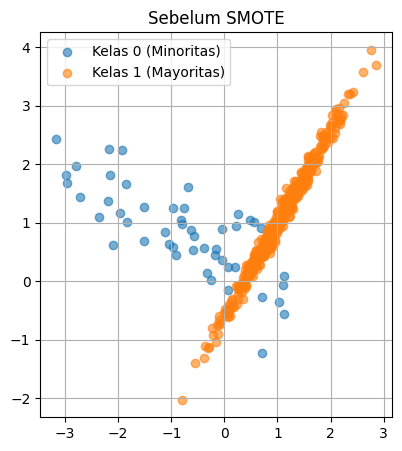
\includegraphics[width=0.5\textwidth]{figure/visualisasi_data_sebelum_smote.png}
	\caption{Visualisasi Data Sebelum SMOTE}
	\label{fig:2.visualisasidatasebelumsmote}
\end{figure}

\begin{figure}[H]
	\centering
	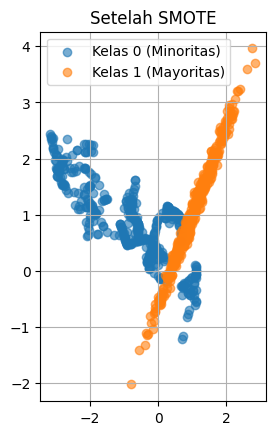
\includegraphics[width=0.5\textwidth]{figure/visualisasi_data_sesudah_smote.png}
	\caption{Visualisasi Data Sesudah SMOTE}
	\label{fig:2.visualisasidatasesudahsmote}
\end{figure}

\subsection{ADASYN (Adaptive Synthetic Sampling)} \label{II.adasyn}
ADASYN (\textit{Adaptive Synthetic Sampling}) adalah teknik yang digunakan untuk menangani ketidakseimbangan(imbalance) kelas dalam tugas klasifikasi, namun dengan pendekatan yang lebih adaptif dibandingkan metode seperti SMOTE\cite{4633969}. ADASYN bekerja dengan membuat sampel sintetis baru untuk kelas minoritas. ADASYN berfokus pada sampel yang sulit untuk diklasifikasikan yang terletak di dekat perbatasan antara kelas mayoritas dan minoritas\cite{4633969}.
\subsubsection{Cara kerja ADASYN}
Berikut cara kerja dibalik ADASYN:
\begin{enumerate}[noitemsep]
    \item Yang pertama ialah tentukan jumlah sampel sintetis yang perlu dibuat untuk setiap sampel minoritas $x_i$ berdasarkan tingkat kesulitan klasifikasi lokal. Tingkat kesulitan lokal $d_i$ dihitung berdasarkan jumlah tetangga terdekat dari kelas mayoritas di sekitar $x_i$.
    \item Yang kedua hitung bobot adaptif atau $r_i$ untuk setiap sampel minoritas $x_i$\\
    yang mana $n_{min}$ adalah jumlah sampel kelas minoritas. Menghitung bobot adaptif ini digunakan untuk menentukan seberapa banyak sampel sintetis yang perlu dibuat untuk setiap sampel minoritas.
    \item Yang terakhir ialah membuat sampel sintetis berdasarkan jumlah total sampel sintetis yang diinginkan. sampel sintetis dibuat dengan menggunakan rumus interpolasi linear SMOTE seperti pada rumus 2.4.\\
\end{enumerate}
Hasil dari metode oversampling ADASYN akan menghasilkan pola data yang berbeda dengan sebelumnya seperti pada gambar \ref{fig:2.visualisasidatasebelumadasyn} menjadi seperti ini pada gambar \ref{fig:2.visualisasidatasesudahadasyn}. Pada gambar \ref{fig:2.visualisasidatasesudahadasyn} dapat dilihat kalau metode oversampling ADASYN membuat data sintetis berdasarkan bobot yang sudah ditentukan sebelumnya dan setalh itu membuat garis interpolasi antar data poin terdekatnya yang mana menghasilkan data sintetis yang banyak namun memiliki data yang cenderung berkumpul pada pertemuan antara data minortas dan mayoritas.

\begin{figure}[H]
	\centering
	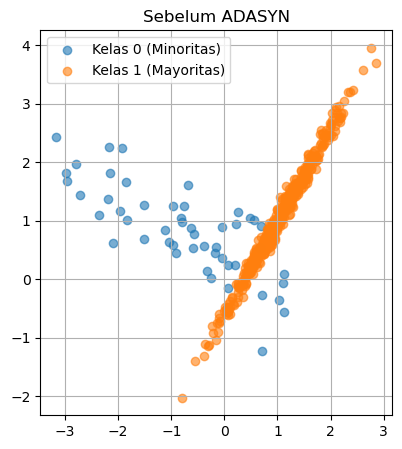
\includegraphics[width=0.5\textwidth]{figure/visualisasi_data_sebelum_adasyn.png}
	\caption{Visualisasi Data Sebelum ADASYN}
	\label{fig:2.visualisasidatasebelumadasyn}
\end{figure}

\begin{figure}[H]
	\centering
	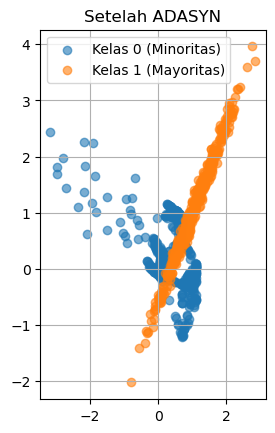
\includegraphics[width=0.5\textwidth]{figure/visualisasi_data_sesudah_adasyn.png}
	\caption{Visualisasi Data Sesudah ADASYN}
	\label{fig:2.visualisasidatasesudahadasyn}
\end{figure}

\subsection{\textit{Decision Tree}} \label{II.decisiontree}
\textit{Decision Tree} merupakan sebuah algoritma machine learning yang digunakan untuk tugas klasifikasi dan regresi dengan memprediksi berdasarkan serangkaian kondisi atau pertanyaan tertentu\cite{song2015decision}. \textit{Decision Tree} sering di visualisasikan dengan gambar pohon terbaik dengan bagian paling atas disebut \textit{root node} dan setiap \textit{node} dibawah \textit{root node} yang ditunjuk oleh panah dan menunjuk panah bisa disebut dengan \textit{decision node atau branches} dan untuk \textit{node} yang hanya ditunjuk dan tidak menunjuk \textit{node} disebut \textit{leaf node}\cite{rojas2012graphical}. Visualisasinya dapat dilihat pada gambar \ref{fig:2.decisiontree}.\\
\begin{figure}[H]
	\centering
	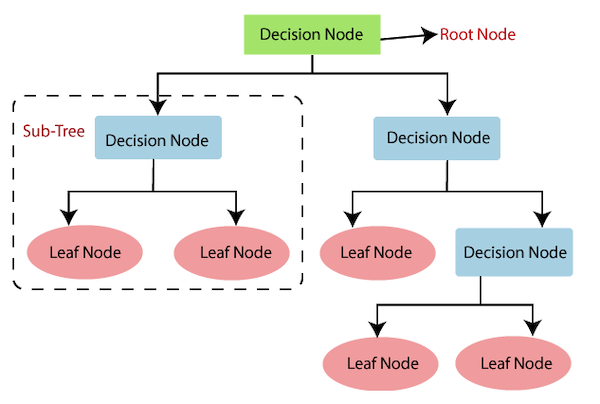
\includegraphics[width=0.5\textwidth]{figure/decision tree.png}
	\caption{Decision Tree}
	\label{fig:2.decisiontree}
\end{figure}
Cara \textit{decision tree} membuat keputusan ialah dengan dengan melakukan perhitungan pada setiap node nya untuk melanjutkan keputusan dengan cara menghitung \textit{gini impurity}, impurity berarti dalam \textit{decision tree} merupakan campuran dari keputusan iya atau tidak dan setelah menghitung gini impurity pada setiap keputusan iya dan tidak, kita hitung \textit{total gini impurity} untuk menjadi ukuran kualitas dari prediksi\cite{suthaharan2016decision}.\\ 
Berikut merupakan rumus \textit{gini impurity}:\\
\begin{equation} 
Gini(D) = 1 - \sum_{i=1}^k [p(i)]^2
\end{equation}
\label{eq:2.gini}
\myequations{Rumus Gini Impurity}\\
Yang dapat kita ketahui bahwa:\\
$D$ = merupakan node.\\
$k$ = merupakan jumlah kelas\\
$p(i)$ = merupakan peluang sampel yang termasuk kelas i pada node.\\
Berikut merupakan rumus dari \textit{total gini impurity}:\\ 
\begin{equation}
Total \ Gini \ Impurity = \sum_{i=1}^n \left[\frac{|D_i|}{|D|} \cdot Gini(D_i)\right]
\end{equation}
\label{eq:2.totalgini}
\myequations{Rumus Total Gini Impurity}\\
Yang mana dapat kita ketahui bahwa:\\
$n$ = merupakan jumlah \textit{node} pada sebuah \textit{tree}\\
$D_i$ = merupakan \textit{dataset} pada \textit{node} i\\
$D$ = merupakan  jumlah total sampel dalam \textit{dataset}\\

\subsection{Random Forest} \label{II.randomforest}
\textit{Random Forest} merupakan algoritma yang dibuat oleh Leo Breiman  yang mana pembuatan random forest ini merupakan lanjutan dari ide paper dia sebelumnya terkait bagging\cite{breiman2001random,breiman1996bagging}.
\textit{Random forest} merupakan salah satu algoritma ensemble learning bertipe \textit{bagging} yang digunakan untuk klasifikasi dan regresi. Algoritma ini bekerja dengan menggabungkan beberapa \textit{decision tree} untuk menghasilkan model yang lebih baik dalam menghindari \textit{overfitting}\cite{breiman2001random}. Setiap tree dalam \textit{random forest} dilatih dengan menggunakan subset data yang berbeda yang kita sebut sebagai \textit{boostrapped dataset} yang mana cara kerjanya cukup sederhana hanya memilih secara acak data yang ada pada original dataset dengan aturan:
\begin{enumerate}[noitemsep]
    \item Saat pemilihan acak boleh memilih data yang sama yang artinya apabila saat memilih data secara acak itu terpilih data yang sama maka itu diperbolehkan.
    \item Ukuran dari \textit{boostrapped dataset} itu harus sama dengan original dataset.
\end{enumerate}
Setelah membuat \textit{boostrapped dataset} akan dilakukan pembuatan decision tree dengan menggunakan boostrapped dataset, dalam pembuatan decision tree kita perlu menentukan berapa \textit{max feature} yang kita pilih secara acak pada setiap \textit{split tree}.\\
setelah pembuatan tree selesai dilakukan maka kita mengulang proses tersebut hingga ratusan kali atau sesuai yang kita yang tentukan dan keputusan akhir dibuat dengan menggabungkan hasil dari semua \textit{tree} sepeti pada gambar \ref{fig:2.randomforest}.\\
\begin{figure}[H]
	\centering
	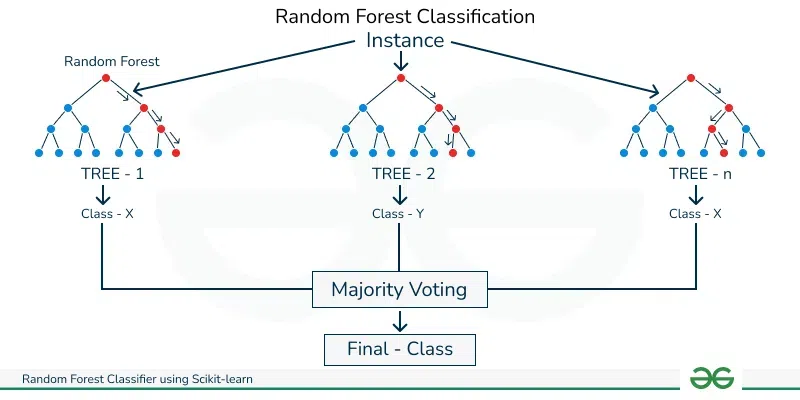
\includegraphics[width=0.7\textwidth]{figure/random_forest.png}
	\caption{Random Forest}
	\label{fig:2.randomforest}
\end{figure}
\textit{Random forest} memikiki banyak \textit{hyperparameter} yang digunakan untuk mengatur bagaimana random forest bekerja. \textit{Hyperparameter} yang digunakan dalam \textit{random forest} ialah sebagai berikut.
\begin{enumerate}[noitemsep]
    \item n\_estimator digunakan untuk menentukan seberapa banyak \textit{tree} yang ingin digunakan pada model \textit{random forest}.
    \item max\_depth digunakan untuk menentukan maksimum kedalaman \textit{tree}.
    \item min\_sample\_split digunakan untuk menentukan jumlah minimum yang dibutuhkan untuk \textit{split} pada \textit{internal node}.
    \item min\_sample\_leaf digunakan untuk menentukan jumlah \textit{minimum} yang dibutuhkan untuk membuat \textit{leaf node}.
    \item max\_feature digunakan untuk menentukan seberapa banyak \textit{feature} yang dibutuhkan pada setiap \textit{split}.
    \item bootstrap digunakan untuk menentukan apakah menggunakan \textit{boostrap sampling} atau tidak untuk membuat \textit{training set} pada setiap \textit{tree}.
\end{enumerate}

\subsection{XGBoost} \label{II.xgboost}
Extreme Gradient Boosting atau XGBoost adalah salah satu ensemble learning bertipe boosting dan merupakan sebuah algoritma \textit{machine learning} yang dioptimalkan untuk implementasi metode \textit{gradient boosting}\cite{chen2015xgboost}. Algoritma ini dikenal karena kecepatannya, efisiensinya, dan kemampuannya menghasilkan model yang sangat akurat, sehingga sering digunakan dalam kompetisi pembelajaran mesin seperti yang diadakan di platform Kaggle.
\textit{XGBoost} digunakan untuk menyelesaikan masalah klasifikasi dan regresi\cite{chen2016xgboost}.\\
\textit{XGBoost} memikiki banyak \textit{hyperparameter} yang digunakan untuk mengatur bagaimana xgboost bekerja. \textit{Hyperparameter} yang digunakan dalam \textit{xgboost} ialah sebagai berikut\cite{xgboost_parameter_documentation}:
\begin{enumerate}[noitemsep]
    \item max\_depth digunakan untuk menentukan maksimum kedalaman \textit{tree}.
    \item learning\_rate digunakan untuk menentukan seberapa banyak step yang dilakukan pada setiap iterasi.
    \item n\_estimator digunakan untuk menentukan seberapa banyak tree yang ingin digunakan pada model xgboost.
    \item min\_child\_weight digunakan untuk menentukan jumlah bobot minimum yang digunakan dalam \textit{child node}.
    \item subsample digunakan untuk mengontrol seberapa banyak bagian \textit{training instances} yang digunakan pada setiap tree didalam xgboost.
    \item colsample\_bytree digunakan untuk mengontrol seberapa banyak \textit{feature} yang dipilih secara \textit{random sample} pada setiap \textit{tree} saat \textit{training}.
    \item gamma digunakan untuk menentukan minimum dari \textit{loss reduction} yang dibutuhkan untuk split \textit{tree}.
    \item alpha digunakan untuk mengontrol \textit{L1 regularization}.
\end{enumerate}

\subsection{Evaluasi Model} \label{II.evaluasimodel}
Pengujian model pada penelitian ini dengan membandingkan hasil test \textit{precision}, \textit{recall}, \textit{f1-score}, dan \textit{Matthews’s correlation coefficient} (MCC) \textit{metrics} untuk mendapatkan hasil terbaik. Untuk mendapatkan pengukuran tersebut dibutuhkan \textit{confusion matrix} seperti berikut.
\begin{figure}[H]
	\centering
	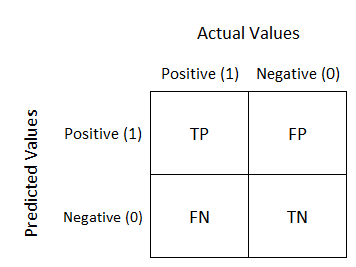
\includegraphics[width=0.5\textwidth]{figure/confusion_matrix.png}
	\caption{Confusion Matrix}
	\label{fig:2.confusionmatrix}
\end{figure}
yang mana \textit{confusion matrix} dibagi menjadi 4 yaitu:
\begin{enumerate}[noitemsep]
    \item True Positive (TP), jumlah data prediksi positif yang terdeteksi benar.
    \item True Negative (TN), jumlah data prediksi negatif yang terdeteksi benar.
    \item False Positive (FP), jumlah data prediksi negatif yang terdeteksi data positif.
    \item False Negative (FN), jumlah data prediksi positif yang terdeteksi data negatif.
\end{enumerate}
Barulah berdasarkan \textit{confusion matrix} kita dapat menghitung \textit{precision}, \textit{recall},     \textit{f-1 score}, dan \textit{Matthews’s correlation coefficient} (MCC) \textit{metrics}.

\subsubsection{Precision}
\textit{Precision} adalah perbandingan antara jumlah prediksi positif yang benar(TP) dengan total jumlah prediksi positif(TP + FP). \textit{Precision} menunjukan seberapa seberapa akurat model dalam memprediksi kelas positif. \textit{Precision} digunakan untuk menjawab pertanyaan seperti "dari semua \textit{instances} yang diprediksi positif, berapa banyak yang benar-benar positif?". \textit{Precision} dihitung dengan formula seperti berikut:\\
\begin{equation}
Precison = \frac{TP}{TP + FP} 
\end{equation}
\label{eq:2.precision}
\myequations{Rumus Precision}\\
Kegunaan dari \textit{precision} itu sangat penting dalam kasus dimana false positive tinggi. Contohnya dalam pendeteksi penipuan kartu kredit, kita ingin mengurangi kemungkinan mendeteksi transaksi yang tidak penipuan namun dikategorikan sebagai transaksi penipuan.
   
\subsubsection{Recall}
\textit{Recall} adalah perbandingan antara jumlah prediksi positif yang benar(TP) dengan total jumlah data aktual yang positif(TP+FN). \textit{Recall} menunjukkan seberapa baik model dalam menangkap semua data positif yang ada. \textit{Recall} digunakan untuk menjawab pertanyaan seperti "Dari semua kejadian yang benar-benar positif, berapa banyak yang diprediksi positif dengan tepat?". \textit{Recall} dapat dihitung dengan formula seperti berikut:\\
\begin{equation}
Precison = \frac{TP}{TP + FN} 
\end{equation}
\label{eq:2.recall}
\myequations{Rumus Recall}\\
Kegunaan dari \textit{recall} ialah pada kasus dimana memerlukan deteksi penyakit kita ingin recall yang tinggi untuk menangkap semua kasus penyakit agar tidak ada pasien yang tidak terdiagnosis. Recall berfokus pada  memastikan bahwa semua kasus positif terdekteksi meskipun ada beberapa kesalahan \textit{false positive} sedangkan \textit{precision} berguna ketika penting untuk memastikan bahwa prediksi benar-benar akurat, sehingga mengurangi jumlah \textit{false positive}.


\subsubsection{F1-Score}
\textit{F1-Score} adalah rata-rata harmonik dari precision dan recall. \textit{F1-Score} memberikan keseimbangan antara precision dan recall yang berguna saat ada ketidakseimbangan kelas.\\
\begin{equation}
F1-Score = 2 \times \frac{Precision \times Recall}{Precision + Recall}   
\end{equation}
\label{eq:2.f1score}
\myequations{Rumus F1 Score}\\
Kegunaan dari \textit{f1-score} ialah pada situasi dimana penting untuk menjaga keseimbangan antara \textit{precision} dan recall, untuk menghindari bias terhadap kelas mayoritas.    

\subsubsection{Matthews correlation coefficient}
\textit{Matthew’s Correlation Coefficient} 
(MCC) adalah ukuran evaluasi yang digunakan untuk mengukur kinerja sebuah model dalam melakukan klasifikasi biner. MCC berkerja dengan mempertimbangkan semuan nilai yang ada dalam \textit{confusion matrix}(TP, TN, FP, FN) dalam menggambarkan hasil kualitas prediksi model, dikarenakan mcc mempertimbangkan semua elemen yang ada pada confusion metrix maka mcc dapat dijadikan sebuah metrik evaluasi yang baik untuk kelas yang tidak seimbang(\textit{unbalance})\cite{chicco2020advantages}. MCC dapat dihitung dengan formula seperti berikut:\\
\begin{equation}
MCC = \frac{(TP \times TN) - (FP \times FN)}{\sqrt{(TP + FP)(TP + FN)(TN + FP)(TN + FN)}} 
\end{equation}
\label{eq:2.mcc}
\myequations{Rumus Matthews correlation coefficient}\\
Hasil dari nilai \textit{matthew’s Correlation Coefficient} diinterpretasikan sebagai
\begin{enumerate}[noitemsep]
    \item +1: Model membuat prediksi sempurna (semua prediksi benar).
    \item 0: Model tidak bisa melakukan prediksi dan sama seperti tebakan acak.
    \item 1: Model membuat prediksi yang salah secara total.
\end{enumerate}
Pada penelitian ini juga peneliti akan menggunakan mcc sebagai metrik utama untuk menentukan gambaran performa model dan peneliti tidak akan menggunakan roc auc disebabkan semakin tinggi hasil dari mcc(contoh: MCC = 0.9) maka semakin tinggi pula nilai roc auc namun tidak sebaliknya\cite{chicco2023matthews}.


